\documentclass[12pt,a4paper]{scrartcl}
\usepackage[top=2cm,bottom=2cm,left=2cm,right=2cm]{geometry}
\usepackage[ngerman]{babel}
\usepackage[utf8]{inputenc}
\usepackage{listings}
\usepackage{graphicx}
\usepackage{wrapfig}
\usepackage{tabularx}
\usepackage{xcolor}

\graphicspath{../.}

\newcommand{\glsref}[1]{\textit{\textbf{#1}}}

\lstset{
	basicstyle=\small,
	tabsize=4,
	literate={ä}{{\"a}}1 {ö}{{\"o}}1 {ü}{{\"u}}1 {Ä}{{\"A}}1 {Ö}{{\"O}}1 {Ü}{{\"U}}1 {ß}{{\ss}}1 
}

\begin{document}
\title{Entwicklung und Implementierung eines Netzwerkprotokolls zur bidirektionalen Kommunikation und Fernsteuerung eines Systems unter Zuhilfenahme einer selbstentwickelten Sprache zur Programmsteuerung}
\date{Januar 2019}
\author{\hfill\\ 
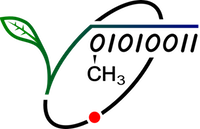
\includegraphics[scale=2.5]{logo}\hfill\\\hfill\\\hfill\\\hfill\\\textbf{Leonard Petereit}\\\textbf{Benedikt Schäfer}\\\hfill\\\hfill\\
\textbf{Fachbetreuung - Herr J. Süpke}\\
\textbf{Seminarfachbetreuung - Frau Dr. M. Moor}
\hfill\\\hfill\\\hfill\\
}
\clearpage\maketitle
\thispagestyle{empty}
\newpage
\tableofcontents
\thispagestyle{empty}

\newpage
\documentclass[12pt,a4paper]{scrartcl}

\usepackage[ngerman]{babel}
\usepackage[utf8]{inputenc}

\begin{document}
\section*{Einleitung}
Daten speichern und verwalten ist eine komplexe Aufgabe, die viele kleine Probleme beinhaltet. So zum Beispiel das Bereitstellen von genug Speicherplatz oder das Verschieben, Kopieren, Umbenennen, Auslesen oder Sichern der Daten; letzteres soll oft von jedem beliebigen Ort aus möglich sein, da man nicht nur zu Hause auf z.B. Urlaubsbilder, Musik und Videos zugreifen will; hat man viele\\
Die einfache Lösung würde darin bestehen, den Computer zu Hause fernzusteuern - das ist aber entweder umständlich mit Funktionen des Betriebssystems zu realisieren - was bei verschiedenen Betriebssystemen noch problematischer wird - oder mit schlecht erweiterbaren grafischen Systemen, die einen fortgeschrittenen Nutzer oft nicht zufrieden stellen.
Ein auf einer Ebene dazwischen angesiedeltes System zur Fernsteuerung wäre sinnvoll - also eine betriebssystemunabhängiges Software zur Versendung von Steuerbefehlen an einen über ein Computernetzwerk verbundenen Zielcomputer mit der Möglichkeit Dateien zu übertragen, welches den Nutzer in seinen Möglichkeiten nicht beeinträchtigt und trotzdem eine nicht überladene Oberfläche besitzt - das ist unsere Zielstellung.
%kp, mal irgendwann weiterschreiben

Dieses grob formulierte Ziel schlüsselt sich auf in mehrere Unterprobleme. Als Grundlage soll ein Netzwerkprotokoll entwickelt werden, welches unseren gestellten Ansprüchen gerecht erstellt werden muss. Es sollte also optimiert sein für die Übertragung von Anweisungen eines vom Nutzer erweiterbaren Satzes und Dateien jeglichen Typs; dabei muss es sicherstellen, dass die Daten sicher und fehlerfrei, sowie im richtigen Format ankommen.\\
Die Kommunikation mit dem Nutzer geschieht über ein Terminal; die Eingabebefehle sind Teil einer selbst definierten formalen Sprache - damit werden unkomplizierte Bedienung und eine Möglichkeit zur Erweiterung kombiniert.
Es soll dem Nutzer möglich sein, den vorhandenen Kanon an Befehlen und Argumenten beliebig zu erweitern, ohne das gesamte Programm neu kompilieren zu müssen. Deshalb wird die gesamte Eingabeverarbeitung intern von einer Implementierung durch eine Skriptsprache geregelt.\\
Zu guter Letzt muss unser Programm modular aufgebaut sein, damit es von allen drei Mitgliedern von den Schnittstellen abgesehen unabhängig entwickelt werden kann.
%meh. wird irgendwie nicht mehr xD
% ^+1 später... 

\end{document}
\setcounter{page}{1}


\newpage

%\documentclass[12pt, a4paper]{scrartcl}
%\usepackage[german]{babel}
%\usepackage[utf8]{inputenc}
%\usepackage{graphicx}
%
%\usepackage{listings}
%
%\begin{document}
\section{Funktionsumfang und Eingabeverarbeitung auf der Anwendungsebene}

\subsection{Entwicklung einer eigenen Scriptsprache zur Anwendungssteuerung}
\subsubsection{Theoretische Grundlagen formaler Sprachen}
Wir als Menschen haben die gesprochenen Sprachen entwickelt, um uns untereinander zu verständigen und Informationen auszutauschen. Um Missverständnisse zu vermeiden, ist unsere Kommunikation durch strikte grammatikalische und semantische Regeln definiert. Es werden strukturelle Merkmale wie zum Beispiel die Reihenfolge einzelner Sprachteile festgelegt, außerdem gibt es einen begrenzten Wortschatz, indem jedes Wort eine bestimmte Bedeutung hat.
Um auch Computern Informationen zu übermitteln, und eine maschinelle Verarbeitung dieser zu ermöglichen, benutzt man formale Sprachen. Diese gleichen von den grundlegenden strukturellen Ansprüchen den natürlichen Sprachen, verfügen also auch über eine Syntax und eine Semantik, definieren sich allerdings dadurch, dass diese für einen Rechner eindeutig verständlich sein müssen, und demnach kein Interpretationsfreiraum gelassen wird. Ziel ist es klare Anweisungen in einer für den Computer verständlichen Weise zu übermitteln.\\
Da Sprachen in der Regel durch das Aneinanderreihen von einzelnen Sprachelementen über eine Unendlichkeit verfügen, nutzt man künstliche Grammatiken der Form $G = (N, T, P, s)$, um diese zu beschreiben. Eine Grammatik $G$ dieser Art verfügt über eine Menge von nichtterminalen Symbolen $N$, oder auch Variablen genannt, welche im Verlauf der Wortbildung durch die Menge der Produktionsregeln $P$ der Form $U \rightarrow V$ durch eine Kombination aus terminalen Zeichen der Menge $T$ ersetzt werden. Das Startsymbol $s$ ist zwingend die erste Variable, welche durch eine Produktion der Form $s \rightarrow V$ ersetzt wird. Ein Wort gehört einer Grammatik $G$ an, wenn es nur noch aus terminalen Symbolen der Menge $T_G$ besteht und ausgehend von dem Startsymbol $S_G$ mit den Produktionen der Menge $P_G$ gebildet werden kann.\footnote{$	https://www.uni-ulm.de/fileadmin/website_uni_ulm/iui.inst.040/Formale_Methoden_der_Informatik$\\$/Vorlesungsskripte/FMdI-06--2010-01-10--FormaleSprachen_Vorlesung.pdf$
; 19.11.2018}\\
Je nachdem nach welcher Art die Produktionsregeln einer Grammatik aufgebaut sind, lässt sich eine formale Sprache nach dem Informatiker Noam Chomsky in vier Typen einteilen. Grundsätzlich gehört jede Sprache dem Typ 0 der allgemeinen Sprachen an. Eine Sprache gehört immer einem Typ $X$ an, wenn alle Bedingungen  der Typen $\leq X$ für alle Produktionsregeln der Form $U \rightarrow V$ erfüllt sind. Die Bedingung für eine kontextsensitive Sprache des Typs 1 besagt, dass durch eine Produktionsregel das Wort nicht verkürzt werden kann, also $|U| \leq |V|$. Für eine kontextfreie Sprache des Typs 2 gilt, dass durch eine Produktionsregel nur jeweils eine Variable ersetzt werden kann, also $|U| = 1$. Eine Sprache ist eine reguläre Sprache des Typs 3, wenn ein nichtterminales Symbol mit einer Produktionsregel durch ein terminales Symbol und ein optionales nichtterminales Symbol ersetzt wird, jedoch nicht durch mehre, also $U \leq a|aB$. \footnote{I. Wegener;	Theoretische Informatik; Kap.5}\\
\begin{table}[h!]
\begin{tabular}{|ll|ll|}
\hline
Verwendung                    & Zeichen   & Verwendung                    & Zeichen \\ \hline
Definition                    & =         & Aufzählung                    & ,       \\
Endezeichen                   & ;         & Alternative                   & |       \\
Option                        & {[}...{]} & Optionale Wiederholung        & \{...\} \\
Gruppierung                   & (....)    & Anführungszeichen 1. Variante & "..."   \\
Anführungszeichen 2. Variante & '...'     & Kommentar                      & (*...*) \\
Spezielle Sequenz             & ?...?     & Ausnahme                      & -       \\ \hline
\end{tabular}
\end{table}
Um die Darstellung von Sprachen zu vereinheitlichen, wurde die Erweiterte-Backus-Nauer-Form, kurz EBNF entwickelt. Die oben gegebenen Zeichen sind Teil des EBNF ISO-Standards und durch sie lässt sich jede beliebige formale Sprache beschreiben.\\

 
\subsubsection{Spezifikation unserer Skriptsprache anhand unserer Ansprüche an den Funktionsumfang}
Für unser Programm haben wir uns grundlegend vorgenommen, Funktionen für das Versenden von Dateien, sowie Befehlen an einen zweiten PC bereitzustellen. 
Es erfordert also in gewissem Maße eine Kommunikation zwischen dem Nutzer und dem Programm, um die Wünsche des Bedieners genauer zu spezifizieren und der Software zu übermitteln. 
Um dies zu bewerkstelligen entschieden wir uns, eine eigene formale Sprache zu entwickeln, mit dem Ziel Befehle an das Programm mit den entsprechenden Argumenten zu übermitteln, welche über ein Konsolenfenster eingegeben werden.
Unsere Sprache sollte Folgende Anweisungen beinhalten:\\
\begin{table}[h!]
\centering
\begin{tabular}{|ll|}
\hline
Befehl & Argumente \\ \hline
send\_file & file\_name file\_type \\
send\_comm & comm\_name {[}arguments{]} \\
get\_file & file\_name file\_type \\
connect & ip\_address [port]\\
disconnect & \\
reconnect & ip\_address [port]\\
shutdown [send\_comm] & \\
open [send\_file] & file\_name file\_type \\ \hline
\end{tabular}
\end{table}\\
Die Befehle $send\_file$ und $send\_comm$ sind hierbei die allgemeinen Funktionen zum Senden einer Datei oder eines Befehls an die betriebssystemeigene Kommandozeile, jeglicher Art. Das Kommando $get\_file$ ist identisch zu $send\_file$ mit dem Unterschied, dass eine Datei von dem angefragten PC auf den anfragenden übertragen werden soll. Mit den Anweisungen ($dis-$/$re-$)$connect$ wird der grundlegende Verbindungsaufbau gesteuert. Durch den $connect$-Befehl wird versucht eine Verbindung zu der als Argument übergebene IP-Adresse zu errichten. $disconnect$ bewirkt die Beendigung einer bestehenden Verbindung, $reconnect$ versucht zusätzlich eine neue Verbindung zu erstellen. 
$shutdown$ und $open$ sind spezielle versendete Anweisungen, zum Herunterfahren des Zielcomputers und Öffnen einer Datei, bei denen wir es aufgrund ihrer frequentierten Nutzung für sinnvoll hielten, sie eigenständig in unsere formale Sprache zu integrieren. Sie basieren auf den zwei Grundfunktionen und stehen beispielhaft für die Erweiterbarkeit des Funktionsumfangs unserer Software. 
Zusätzlich für Befehle, welche mit Dateien arbeiten sollen, müssen sowohl der Dateiname als auch das Dateiformat als Zeichenkette angefügt werden. 
Die Übermittlungsfunktionen für Anweisungen benötigt neben dem Anweisungsnamen als Zeichenkette auch optionale Argumente, mit welchem die Anweisung in der Kommandozeile ausgeführt werden soll.\\
Um unsere formale Sprache zu implementieren, entwickelten wir zuerst eine Darstellung der Eweiterten-Backus-Nauer-Form, diese ist im Anhang einzusehen. Eine solche Darstellung hat den Vorteil einer unkomplizierten Übertragung der Produktionsregeln in die Implementierung, welche die Nutzereingaben überprüft.

\subsection{Implementierung der Anwendungssteuerung in der Skriptsprache Lua}

\subsubsection{Darstellung des grundlegenden Programmaufbaus und Programmablaufs}
Grundlegende Aufgabe der Anwendungssteuerung ist es, die Eingaben die der Nutzer unserer Software tätigt, in Aktionen des Programms umzusetzen. Dazu werden zum einen auf dem Rechner der sendenden Person die nach der in Kapitel 3.1 beschriebenen Syntax eingegebene Anweisung, in der Eingabeverarbeitung auf ihre Korrektheit überprüft, um anschließend aufgeschlüsselt zu werden und die gewünschte Sendefunktion zu initialisieren.\\
Nachdem die Daten mithilfe des Netzwerkprotokolls übermittelt wurden, werden sie von der Übertragungsverarbeitung, auf dem Empfängercomputer weiter bearbeitet. Je nach spezifiziertem Typ der Übermittlung, wird entweder die enthaltene Datei auf Fehler überprüft und anschließend endgültig gespeichert, oder die auszuführende Anweisung wird an die betriebsystemeigene Kommandozeile weitergegeben und ausgeführt.\\
Um keine ungewollten Übertragungen von potenziell schädlichen Dateien oder Anweisungen zu ermöglichen, wird für die Ausführung jeder Übermittlungsanfrage die Bestätigung des Empfängers benötigt, sofern nicht der $root-Modus$ aktiviert ist. Als $root$-Nutzer hat man uneingeschränkte Kontrolle über den Ziel-Computer, was besonders für administrative Tätigkeiten sinnvoll ist.\\\hfill\\ 
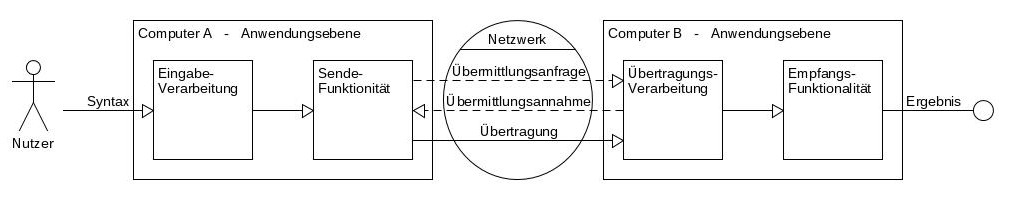
\includegraphics[scale=.45]{anw.jpg}
\subsubsection{Ansprüche an die Implementierung und die daraus resultierende Wahl der Programmiersprache}
Wie in Kapitel 3.2.1 erläutert, wird auf der Anwendungsebene unseres Programmes, also dem Teil welcher nicht für die Kommunikation im Netzwerk zuständig ist, die grundlegende Funktionalität implementiert. Da unser selbstentwickeltes Netzwerkprotokoll, welches die eigentliche Kommunikation zwischen 2 Computern regelt, relativ universell auf verschiedenartige Daten anwendbar ist, stellt dieses im Bezug auf den Funktionsumfang der Software nicht den limitierenden Faktor da. Um das Protokoll eventuell auch im Zeitraum nach der eigentlichen Arbeit ausnutzen zu können, und nicht durch einen festgelegten Satz von Befehlen beschränkt zu werden, entschieden wir uns dazu diesen Programmteil in einer Skriptsprache zu implementieren.
Diese Klasse von Programmiersprachen kennzeichnet sich dadurch aus, dass der vom Menschen lesbare Quelltext eines Programmes erst bei seiner Ausführung in Anweisungen übersetzt werden, welche für den Computer ausführbar sind. Im Gegensatz zu kompilierten Sprachen hat dies den Vorteil, dass Programmcode unkompliziert korrigiert und modifiziert werden kann und sofort lauffähig ist.\\
In diesem Zusammenhang ergibt sich außerdem eine leichte Wartbarkeit, also die Möglichkeit eventuell auftretende Fehler zu beseitigen, als ein weiterer erfüllter Anspruch. Da wir stets zu dritt an unserer Software programmiert haben, sollte es jedem von uns mit möglichst geringem Aufwand möglich sein, Programmteile zu verbessern, auch wenn es sich nicht um den ursprünglichen Autor handelt.\\
Den Vorteil von kompilierten Programmiersprachen, dass sie sich durch eine höhere Leistungsfähigkeit besonders bei komplexeren Problemen auszeichnen, haben wir uns durch die Implementierung unserer Netzwerkteils in der Sprache C++ zu nutzen gemacht. Dies stellt den Anspruch, dass die gewählte Skriptsprache problemlos in Software der Sprache C++ einzubetten ist, und keine Probleme an der Schnittstelle der beiden Programmteile mit zwei unterschiedlichen Sprachen auftreten.\\
Da wir als Gruppenmitglieder unterschiedliche Betriebsysteme auf unseren Arbeitsrechnern benutzen, entstand als Nebenprodukt die Anforderung, dass das finale Programm systemunabhängig sein muss, also ohne erheblichen Aufwand auf neue Betriebssysteme portierbar ist. Unser Fokus lag dabei für die Arbeit auf Computersystemen und wir haben mobile Geräte vorerst außen vor gelassen.
Zu guter Letzt ist der Zeitraum der Seminarfacharbeit auch nur auf eineinhalb Jahre begrenzt, weshalb die gewählte Sprache mit einem geringem Lernaufwand benutzbar sein muss.\\
Als Kompromiss zwischen allen beschriebenen Ansprüchen entschieden wir uns für die Programmiersprache Lua. Da sie in reinem C geschrieben ist, weist sie eine uneingeschränkte Integrationmöglichkeit in bereits vorhandenen C++ - Kontext vor, und lässt sich außerdem auf die am weitesten verbreiteten Betriebssytemarchitekturen wie Windows und Unix portieren.\footnote{www.lua.org/about.html, 17.11.2018} Ein positiver Nebeneffekt dieser Wahl ist die hohe Leistungsfähigkeit von Lua, verglichen zu anderen weit verbreiteten Skriptsprachen. Der Sprachaufbau orientiert sich sehr nah an der Englischen Sprache, was ein schnelles Erlernen ermöglichte.


\subsubsection{Erläuterung wesentlicher Elemente der Implementierung}
Eine zentrale Rolle in der Umsetzung unserer Eingabeverarbeitung spielt die Interpreter-Funktion. Ihre Aufgabe besteht darin, die von dem Nutzer in Form einer Zeichenkette gelieferten Eingabe, in eine für das Programm verständliche Form zu übertragen. Sie ruft außerdem die Funktionen auf, welche die gewünschte Funktionalität implementieren, und übergibt ihnen die eingegebenen Parameter zur weiterführenden Überprüfung.\\\hfill\\
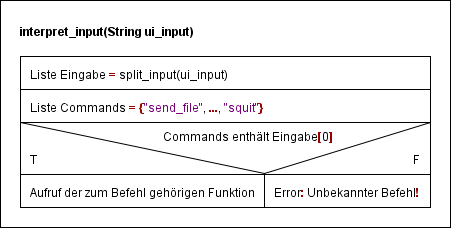
\includegraphics[scale=0.75]{templ}\\
%\begin{lstlisting}[caption = {Interpreter Funktion}]
%function interpret_input(ui_input)
%    local content = split_input(ui_input)
%    local commands = {
%        ["send_file"]=0,
%        ["send_comm"]=0,
%        ["get"]=0,
%        ["open"]=0,
%        ["shutdown"]=0}
%    if commands[content[1]]~=NIL then
%        local result = _G[content[1]](content)
%        print(result)
%    else
%        local name = debug.getinfo(1, "n").name..": "
%        local subject = string.format("%q",content[1])
%        print("ERROR: "..name..subject.." - unbekannter Befehl!")
%    end
%end
%\end{lstlisting}\hfill\\
%TODO es gibt die Variable content nicht im Bild
%TODO was passiert wenn ein String als Argument übergeben wird, der Leerzeichen hat?
Die Variable $content$ (in der Abblidung $Eingabe$ genannt) ist eine Liste der eingegebenen Wörter, sie wird durch die Funktion $split\_input$ erstellt, welche die rohe eingegebene Zeichenkette an den Leerzeichen teilt, und demnach wortweise abspeichert. In der Liste $commands$ wird der Befehlssatz gespeichert, hierbei wird dem Namen von jedem verfügbaren Befehl ein Wert zugeordnet, es spielt keine Rolle welcher Wert es ist, wichtig ist nur, dass die Variablen initialisiert sind und nicht keinen zugeordneten Wert haben. In der folgenden $If-Else$-Struktur wird überprüft, ob der eingegebene Befehl ein Teil des Befehlssatzes ist, sprich ob in der Liste $commands$ ein Wert für den gewünschten Befehl vorliegt. Ist dies nicht der Fall, gibt die Funktion einen Fehler der Form \glqq$ERROR: interpret\_content: EINGABE - unbekannter Befehl!$\grqq\ aus, und es wird keine Übertragung eingeleitet. Wenn die eingegebene Anweisung Teil des Befehlssatzes ist, so wird die entsprechende Funktion mit den übergebenen Parametern aufgerufen, und das Ergebnis in der Variable $result$ gespeichert. Der Aufruf geschieht durch die Lua-Interne Funktion $.G[STRING](ARGUMENTS)$, welche eine Zeichenkette als Input fordert, und eine Funktion dieses Namens mit den gewünschten Argumenten $ARGUMENTS$ aufruft.\\ 
Die gewählte Form der Implementierung, dass der Befehlssatz in einer Liste bestehend aus den Namen der zugehörigen Funktionen, gespeichert ist, ermöglicht eine unkomplizierte Erweiterung der grundlegenden Befehle durch neue Funktionalität, welche möglicherweise spezifischere Ansprüche an das Protokoll fordert. 
Beispiel hierfür ist die Implementierung von Streaming, die einen ständigen Erhalt der Netzwerkverbindung zwischen den zwei Rechnern benötigen würde. \\
Die eigentlichen Funktionen sind alle nach einem ähnlichen Schema aufgebaut. 
Es gibt zwei verschachtelte $If-Else$-Bedingungen die erfüllt werden müssen, um die eigentliche Übertragung auszulösen. 
In der ersten wird überprüft, ob die gewünschte Übertragung Autorisiert ist. 
Dies ist der Fall, wenn auf dem Computer an den die Übertragung gerichtet ist, der Verbindung zugestimmt wurde. 
Die zweite Bedingung prüft, ob die Anzahl der gegebenen Argumente mit der Anzahl an geforderten Argumenten übereinstimmt. 
Schlägt eine der Bedingungen fehl, so wird der Vorgang abgebrochen und eine Fehlermeldung entsprechen der oben dargestellten Form ausgegeben. 
Sind beide Forderungen erfüllt, werden die Argumente, welche als Zeichenkette eingegeben wurden, in die notwendigen Datentypen konvertiert und die zu den Funktionen zugehörigen Anbindungen an das Netzwerkprotokoll initialisiert.  \\\hfill\\
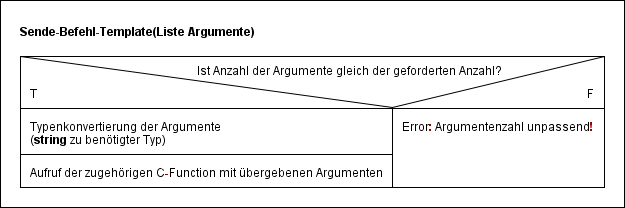
\includegraphics[scale=0.75]{inp}\\
%\begin{lstlisting}[caption = {Beispielhafte Sende Funktion}]
%function send_NAME(args)
%local name = debug.getinfo(1, "n").name
%    if get_length(args)==INTEGER then
%        local ARG1 = args[2]
%        ...
%        local ARGN = args[N+1]
%        if authenticate(ip) then
%            local blank = "c_sendNAME(ARG1, ..., ARGN))"
%        else
%        	local type = " - Uebertragung wurde abgelehnt"
%            print("ERROR: "..name..type)
%        end
%    else
%    	local type = " - Argumentenzahl unpassend"
%        print("ERROR: "..name..type)
%    end
%end
%\end{lstlisting}
%\newpage

%\end{document}


\newpage

%\documentclass[12pt, a4paper]{scrartcl}
%\usepackage[ngerman]{babel}
%\usepackage[utf8]{inputenc}

%\begin{document}
\section{Entwurf und Umsetzung der Netzwerk-Schnittstelle}
\subsection{Grundlegende Theorie zur Kommunikation in einem Netzwerk}
Unter dem Begriff Netzwerk im Zusammenhang mit dieser Arbeit wird, sofern es nicht ausdrücklich anders definiert ist, die Ansammlung mehrerer, untereinander verbundener Computer verstanden.
Diese haben die Möglichkeit mit standardisierten Internet-Netzwerkprotokollen miteinander zu kommunizieren.\\
Diese Kommunikation wird beschrieben durch das ISO/OSI Modell (s. \glsref{ISO/OSI Modell}) der Netzwerkkommunikation, auf dem auch die Arbeitsweise unseres Programmes aufbaut.
Dabei kann man den Prozess, welcher bei einer Netzwerkübertragung abläuft und die verwendeten Informationen in Schichten nach ihrem Abstraktionsgrad einteilen, von Nullen und Einsen in einem Kabel bis hin zu z.B. verschiedensten Verschlüsselungsprotokollen; was in unteren Schichten abgesichert ist, muss in denen darüber nicht implementiert werden, was wiederum zu einfachen und verlässlichen einzelnen Algorithmen in einer Schicht führt, obwohl das gesamte System überaus komplex ist.

\subsection{Notwendigkeit, Anforderungen und Spezifikation eines eigenen Netzwerkprotokolls}
Um das Programm zu dritt zu entwickeln, muss eine gewisse Modularität gewährleistet werden, außerdem müssen die Sinnabschnitte klar nach ihrer Funktion gegliedert sein und leicht benutzbare sowie wiederverwendbare Schnittstellen besitzen, damit nicht das gesamte Programm angepasst werden muss, wenn ein Teil geändert wird und jeder sich auf seinen Teil konzentrieren kann, ohne die anderen vollständig zu kennen.
Diese Anforderungen werden durch die Trennung der Programmiersprachen Lua und C++ einfach geregelt, aber in reinem C++ Kontext muss es dennoch eine Unterteilung zwischen Netzwerkschnittstelle und Benutzeroberfläche geben, weshalb die gesamte Netzwerkkommunikation über eine statische Bibliothek in die ausgeführte Datei eingebunden ist, in dem die Benutzeroberfläche und die Verbindung der Programmteile gemacht werden.
Die Aufgabe der Bibliothek ist, Funktionen und Klassen bereitzustellen, die eine verlässliche Verbindung zwischen zwei Rechnern aufbauen (Start und Ziel), über die ein fester Satz von Anweisungen mit optionalen Argumenten sowie Dateien bidirektional übertragen werden können.
Dafür stellen sich folgende Anforderungen, es muss:

\begin{itemize}
\item ein gesicherter Transport von beliebigen Daten möglich sein,
\item eine verschlüsselte Kommunikation vorliegen
\item der Datenverkehr so klein wie möglich sein
\item der Kommunikationskanal in beide Richtungen gleich aufgebaut sein und
\item die Übertragung auch von größeren Dateien mit zusätzlichen Informationen fehlerfrei ablaufen
\end{itemize}

Diese Bedingungen implizieren bereits, dass eine bestimmte Regelung und einen Ablauf für die Kommunikation zwischen den beiden Computern geben muss: ein Protokoll (s. \glsref{Protokoll}).\par
Alle oben genannten Anforderungen müssen durch dieses Protokoll erfüllt sein und geregelt werden; daher umfasst es sowohl einen bestimmten Datensatz, der in den Header (s. \glsref{Header}) eines Pakets (s. \glsref{Paket}) geschrieben wird als auch einen festgelegten Ablauf der Kommunikation, der sicherstellt, dass alle Daten korrekt ankommen sind und verarbeitet werden.\par 
Um nicht ebenfalls für die Ankunft der Daten selbst sorgen zu müssen, baut das Protokoll auf TCP/IP auf (genauer auf dem Protokoll TLS, welches auch sogar schon eine verschlüsselte Verbindung bereitstellt), also der Transportschicht des ISO/OSI-Modells, auf der bereits genau das implementiert und standardisiert ist - praktisch ist unser Protokoll also auf der Anwendungsschicht des Modells.
Da das Protokoll sowohl für den Versand von Anweisungen als auch für den von Dateien geeignet sein muss und dabei so strukturiert und einfach wie möglich soll, gibt es zwei verschiedene Teilprotokolle, was in folgendem Aufbau der Kommunikationsstruktur resultiert:\par
Im ersten Schritt werden zwei Informationen, als Zahlen codiert, zum Typ der Übertragung, also Anweisung oder Datei, und zu ihrer Gesamtgröße in den Header des ersten Pakets der Übertragung geschrieben.
Abhängig davon, was der Übertragungstyp ist, wird nun entweder die Informationen für eine Dateiübertragung oder eine Anweisungsübertragung angehängt.
Dabei sind alle Werte, sofern es möglich ist, als Zahlen und nicht als Zeichenketten vorhanden, um die Größe der Informationen zu minimieren.\\\par
Betrachtet man zunächst den Header für die Anweisungen, so braucht man einen Anweisungscode, der am Zielort eindeutig zu einer Anweisung zugeordnet werden kann; Teil zwei sind Standardargumente, die binär auf 32 Bit Speicherbreite gespeichert werden.
Dabei soll zum Beispiel, wenn das erste Bit auf eins gesetzt wurde, die Anweisung "`Rufe eine Liste der Daten ab, auf die das Programm Zugriff hat"' nur die Ordnerstruktur herüberschicken, ist das zweite Bit auf eins gesetzt soll es zusätzliche Informationen zur Größe oder den Zugriffsrechten auf die Dateien mitsenden; dafür wären anderenfalls eigene Anweisungen nötig, was der Übersichtlichkeit bei der Implementierung abträglich wäre und deshalb bereits im Protokoll integriert ist.\par 
Der dritte Wert im Headersegment für die Anweisungen ist eine Zahl, die ein Programm identifiziert, auf dass die Anweisung angewendet werden soll, was standardmäßig das Eigene ist.

\begin{figure}[h]
\begin{lstlisting}
     0                   1                   2                   3
     0 1 2 3 4 5 6 7 8 9 0 1 2 3 4 5 6 7 8 9 0 1 2 3 4 5 6 7 8 9 0 1
    +-+-+-+-+-+-+-+-+-+-+-+-+-+-+-+-+-+-+-+-+-+-+-+-+-+-+-+-+-+-+-+-+
    |                        Anweisungscode                         |
    +-+-+-+-+-+-+-+-+-+-+-+-+-+-+-+-+-+-+-+-+-+-+-+-+-+-+-+-+-+-+-+-+
    |                       Standardargumente                       |
    +-+-+-+-+-+-+-+-+-+-+-+-+-+-+-+-+-+-+-+-+-+-+-+-+-+-+-+-+-+-+-+-+
    |                        Zielprogramm-ID                        |
    +-+-+-+-+-+-+-+-+-+-+-+-+-+-+-+-+-+-+-+-+-+-+-+-+-+-+-+-+-+-+-+-+
    |             Länge des optionalen Arguments in Byte            |
    +-+-+-+-+-+-+-+-+-+-+-+-+-+-+-+-+-+-+-+-+-+-+-+-+-+-+-+-+-+-+-+-+
    |              optionales Argument variabler Länge              |
    +-+-+-+-+-+-+-+-+-+-+-+-+-+-+-+-+-+-+-+-+-+-+-+-+-+-+-+-+-+-+-+-+
\end{lstlisting}
\caption{Header für Anweisungen}
\label{Anweisungs_Header}
\end{figure}

Der vierte Wert ist eine Längenangabe in Bytes.
Er bezeichnet die Länge eines optionalen Argumentes, welches an den Header angehängt werden kann, beispielsweise ein Dateiname, eine Chat-Nachricht oder ein Bash-Befehl.\par 
Um die ganze Anweisung klein zu halten wird intern festgelegt, dass die Gesamtgröße dieses Headersegments inklusive des optionalen Arguments nicht größer als $2^{16}$ Byte sein darf - größere Anhänge müssen als Datei verschickt werden.
Aus Kompatibilitätsgründen mit verschiedenen Compilern und Systemen sind alle Werte Integer mit 32 bzw. 64 Bit Speicherbreite, um damit sowohl genügend Platz für alle Informationen zu bieten als auch Probleme mit verschiedenen Rechnerarchitektur-spezifischen Anpassungen der Speicherbreite zu vermeiden.
Insgesamt ergibt sich also die in Abbildung \ref{Anweisungs_Header} zu sehende Spezifikation des Headers für die Versendung von Anweisungen.
Dabei ist die Länge der Argumente in (pro Zeile 32) Bit angegeben, sofern nicht anders spezifiziert.\\\\

\begin{figure}[h]
\begin{lstlisting}
	0                   1                   2                   3
    0 1 2 3 4 5 6 7 8 9 0 1 2 3 4 5 6 7 8 9 0 1 2 3 4 5 6 7 8 9 0 1
   +-+-+-+-+-+-+-+-+-+-+-+-+-+-+-+-+-+-+-+-+-+-+-+-+-+-+-+-+-+-+-+-+
   |                           Dateiart                            |
   |                                                               |
   +-+-+-+-+-+-+-+-+-+-+-+-+-+-+-+-+-+-+-+-+-+-+-+-+-+-+-+-+-+-+-+-+
   |                 Länge des Dateinamens in Byte                 |
   |                                                               |
   +-+-+-+-+-+-+-+-+-+-+-+-+-+-+-+-+-+-+-+-+-+-+-+-+-+-+-+-+-+-+-+-+
   |                  Länge der Prüfsumme in Byte                  |
   |                                                               |
   +-+-+-+-+-+-+-+-+-+-+-+-+-+-+-+-+-+-+-+-+-+-+-+-+-+-+-+-+-+-+-+-+
\end{lstlisting}
\caption{Header für Dateiübertragungen}
\label{Datei_Header}
\end{figure}

Das Versenden von Dateien hat andere Anforderungen, was in einem anderen Aufbau des Header-Segments für eine solche Übertragung, sowie in einem anderen Ablauf resultiert.\par
Für jede Dateiübertragung wird, im Gegensatz zu den Anweisungen, jeweils eine neue TLS-Verbindung aufgebaut(Schritt 0), die unabhängig von vorhergehenden und nachfolgenden ist, es gibt also für jede Datei einen abgeschotteten "`Kanal"', in dem Fehler leicht behandelbar und konkurrierende Übertragungen unmöglich sind; außerdem wird die Kennzeichnung einzelner Datenpakete gespart, was wiederum zu insgesamt weniger Datenverkehr führt.
Danach wird ein Paket mit Informationen zu der Datei zum Zielcomputer geschickt(Schritt 1), welcher, um die Integrität der Übertragung zu verifizieren, dasselbe Paket zurücksendet(Schritt 2).\\

\begin{wrapfigure}{r}{.65\textwidth}
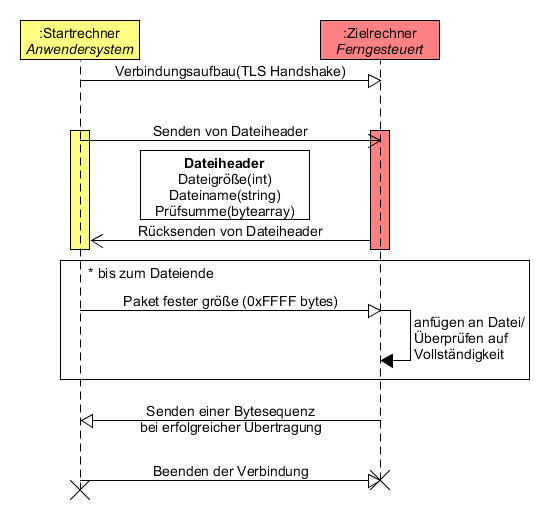
\includegraphics[scale=.4]{diagramFileProtocol}
\caption{Schematische Darstellung des Ablaufs bei der Dateiübertragung}
\label{file_diagram}
\end{wrapfigure}

Dieses Informationspaket ist in Abbildung \ref{Datei_Header} schematisch dargestellt.
Es besteht aus der Art der Datei (z.B. Video, Audio, Text, ausführbare Dateien etc.), was in der weiteren Einordnung im Zielcomputer nützlich ist, dem ursprünglichen Dateinamen und einer Prüfsumme, mit der die fehlerfreie Ankunft verifiziert werden kann.\\
Das Headersegment ist daher so aufgebaut, dass zunächst die drei Ganzzahlwerte für Typ, Länge des Dateinamen in Byte und Länge der Prüfsumme in Byte in den Header geschrieben werden. Dann werden Dateinamenslänge und Prüfsumme angehängt und dieses gesamte Paket wird an den Zielcomputer übermittelt.\par
Ist die Verbindung verifiziert, wird mit der eigentlichen Übertragung der Datei begonnen, die in kleinen Abschnitten und ohne weitere Kennzeichnung in mehreren kleinen Paketen geschieht(Schritt 3 bis x).
Das funktioniert, da unser Standard zum Einen auf TCP/IP aufbaut, welcher bereits die richtige Reihenfolge und Vollständigkeit der Pakete weitgehend sicherstellt und zum Anderen nur eine Verbindung pro Dateiübertragung aktiv ist.
Am Zielcomputer wird die Datei schließlich in einem temporären Standardverzeichnis abgespeichert und Paket für Paket zusammengesetzt.
Ist die Übertragung nach dem Senden einer bestimmten Bytesequenz vom Zielcomputer beendet, wird ein Signal aus der Managerklasse ausgesendet und die Verbindung getrennt.
Diese Schrittfolge ist schematisch in Abbildung \ref{file_diagram} dargestellt.
Nach dem erfolgreichen Übertragen wird noch mit der anfänglich verschickten Prüfsumme der Datei die Integrität der Datei geprüft, um Fehler insgesamt auszuschließen.

\subsection{Funktionsumfang der selbstgeschriebenen Klassenbibliothek}
Die Bibliothek stellt auf oberster Ebene eine Schnittstelle zum Übertragen von Dateien und Anweisungen zu einer bekannten Adresse, welche in angemessener Form codiert sind.
Das heißt konkret, es werden Methoden bereitgestellt, welche die einzelnen Informationen in das passende Format das einfach verschickt werden kann umwandeln, dargestellt durch zwei Klassen, die die nötigen Informationen, also z.B. Dateiprüfsummen, Dateinamen, Anweisungen usw., so verpacken, dass diese dann einfach vom darunterliegenden System verarbeitet werden können.
Zusätzlich dazu ist natürlich eine entsprechende Fehlerbehandlung bei Verbindungsabbrüchen oder fehlerhaften Übertragungen und die Möglichkeit eine Fortschrittsmeldung bei der Dateiübertragung implementiert.
Insgesamt muss der Programmierer nur mit zwei Klassen interagieren, um die volle Funktionalität der Bibliothek ausnutzen, was das gesamte Konstrukt sehr gut für weitere Verwendungen in flexiblen Kontexten der modularen Programmierung eignet und gute Modularität bietet.

\subsection{Implementierung und Funktionsweise der Klassenbibliothek}

\begin{wrapfigure}{r}{.55\textwidth}
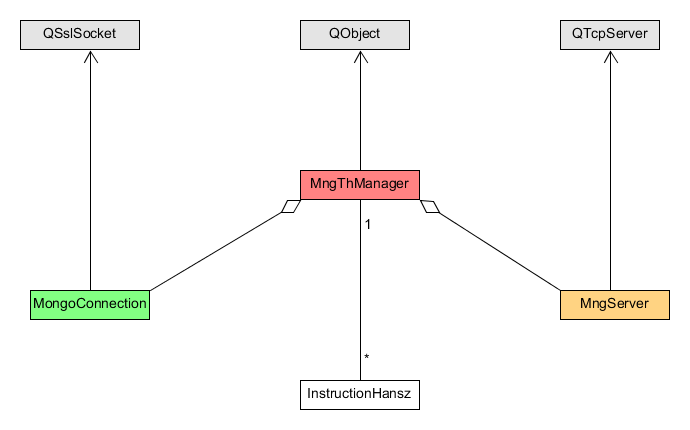
\includegraphics[scale=.4]{classDiagInstr}
\caption{Schematisch: Anweisungsversand}
\label{inst_d}
\end{wrapfigure}

In der Bibliothek sind neben den beiden oben beschriebenen Manager-Klassen (MngThManager für Dateien und MngFileManager für Dateien) mehrere andere Klassen definiert, welche von den jeweiligen Manager-Klassen aus aufgerufen und benutzt werden und dadurch eine darunterliegende Schicht bilden, die durch eine fest definierte Schnittstelle an den Rest des Programms angebunden werden.
Außerdem gibt es eine von allen Klassen benutzte Datei, in denen die Datenstrukturen und Datentypen, die in den Header der Pakete geschrieben werden, als C-Structs definiert sind und einige Funktionen, die häufig gebraucht werden (z.B. String-Vervielfältigung, eine hexadezimale Ausgabe und eine Funktion zum errechnen der Dateiprüfsumme) deklariert; die Definition erfolgt in einer zugehörigen Datei.\par
Der Aufbau der Übertragung beider Datentypen, die verschickt werden, ähnelt sich bis zu einem gewissen Punkt - so haben beide eine eigene Klasse, in der intern die Objekte(Anweisungen und Dateizugriffsobjekte) gespeichert sind und verwaltet werden: (\textit{FileHansz} bzw. \textit{InstructionHansz}), sowie andere Klassen zum Verbindungsaufbau und dem Versand: Eine Klasse, die für das Annehmen von hereinkommenden Verbindungen zuständig ist und eine(bei Dateien zwei) Socket-Klassen, die sich um das Senden bzw. Empfangen von Daten kümmern, was in Abb. \ref{inst_d} bzw. \ref{file_d} vereinfacht schematisch dargestellt ist.\\\\
Die beiden Speicherklassen werden dabei sowohl für den Empfang als auch das Senden eines Objektes genutzt - im ersten Fall werden sie mit den Teildaten(also Anweisungscode und zusätzlichen Argumenten oder Dateiname und Dateityp)
 initialisiert und erstellen daraus einen Pufferspeicher, der bereits den korrekten Header und das Datenpaket enthält, dessen Inhalt dann nur noch ausgelesen und verschickt werden muss - somit ist ein gleicher Aufbau der Verbindung in beide Richtungen sichergestellt.\par
Das tatsächliche Versenden, sowie der Verbindungsaufbau wird von einer "`Server"'-Klasse und den Socket-Klassen übernommen.
Dabei horcht die Serverklasse, sowohl für Dateien als auch für Anweisungen auf der Empfangenden Seite auf einem zuvor bestimmten Port auf eingehende Verbindungen.
Auf der sendenden Seite wird eine neue Klasse erstellt, welche ein TLS-Socket initialisiert und zu der gegebenen Adresse verbindet.
Ist die Verbindungsanfrage eingegangen, wird eine normale TLS-gesicherte Verbindung aufgebaut, sofern das möglich ist; danach weichen die Abläufe von Dateiversand und Anweisungsübertragung ab: Anweisungen werden jetzt, in der Reihenfolge in der sie eingehen, von der Managerklasse an das Socket getaktet weitergeleitet, wo sie dann inklusive Header und Datenpaket verschickt werden - bei Dateien ist der Ablauf etwas komplexer.\par

\begin{wrapfigure}{r}{.55\textwidth}
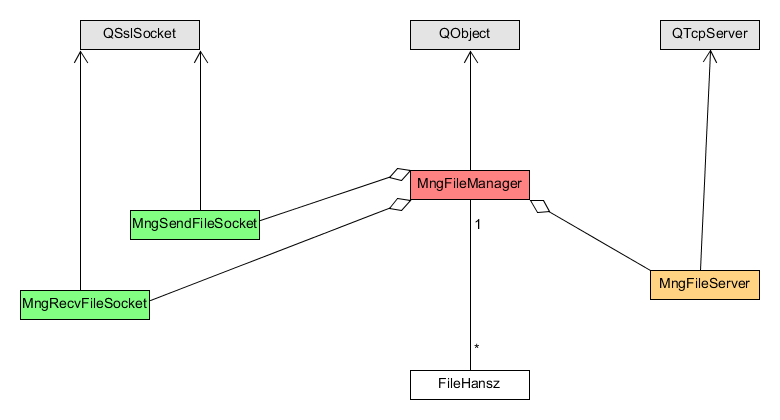
\includegraphics[scale=.35]{classDiagFile}
\caption{Schematisch: Dateiversand}
\label{file_d}
\end{wrapfigure}

Dabei muss zunächst erwähnt werden, dass für Dateien, im Gegensatz zu Anweisungen jedes Mal eine neue Verbindung aufgebaut wird.
In der Verbindung für eine Datei wird, sobald sie aufgebaut ist, zuerst der Header für die Dateiübertragung an den Zielcomputer gesendet(1), welcher genau dasselbe Paket dann zurückschickt(2) um sicherzustellen, dass alle Steuerinformationen korrekt angekommen sind.
Jetzt wird die eigentliche Übertragung der Datei gestartet, welche mit dem Auslesen eines Datenblockes fester Größe beginnt(3).
Dieser wird in einen Pufferspeicher geschrieben, der, wenn er voll ist von der Socket-Klasse ausgelesen und übertragen wird(4); diese Anweisungsfolge(3 und 4) wird so lange wiederholt, bis das Ende der Datei erreicht ist.
Der letzte Datenblock enthält oft weniger als die Maximalgröße, was aber in der Praxis kein Problem ist - das letzte Datenpaket auf der Seite des verschickenden Rechners ist nur etwas kleiner als der Rest.
Auf der empfangenden Seite werden die ankommenden Datenpakete über ihre Repräsentation als FileHansz-Objekt in eine nach der Datei-Prüfsumme benannten Datei im Dateisystem gespeichert - das verhindert die konkurrierende Benennung von ungleichen Dateien und vereinfacht das Überprüfen auf korrekte Übertragung; die ursprünglichen Namen werden zu Beginn der Übertragung per Signal an das Programm außerhalb der Bibliothek geschickt, welches diese dann weitergehend speichert.
Sind alle Pakete versandt worden und angekommen, wofür die TCP-basierte Verbindung sorgt, wird vom Empfangenden Rechner eine Bytesequenz übertragen, welche die Erfolgreiche Übertragung kennzeichnet.\par
Danach wird die Verbindung abgeschlossen und die beiden Sockets gelöscht.\\
%\end{document}

\newpage

%\documentclass[12pt,a4paper]{scrartcl}
%
%\usepackage[ngerman]{babel}
%\usepackage[utf8]{inputenc}

%\begin{document}
\section*{Zusammenfassung}
Unsere grundlegende Zielstellung der Arbeit war es ein Programm zu entwickeln und zu implementieren, welches die Möglichkeiten bereitstellt sowohl Anweisungen als auch Dateien über ein Netzwerk zwischen zwei Computern zu verschicken.\\\\
Zur Verwirklichung dieses Ziels haben wir uns mit dem Design eines eigenen Netzwerkprotokolls beschäftigt, welches die ablaufenden Kommunikationsprozesse zwischen den zwei Rechnern definiert. 
Es baut auf dem gängigen Protokollstandard TLS auf und gliedert die zu übertragenden Daten in eine für unsere Anwendung optimierte Form. 
Zur Nutzereingabe entwickelten wir eine eigene Eingabesyntax auf der Basis einer selbst entwickelten formalen Sprache. 
Im Gegensatz zu natürlichen Sprachen kennzeichnen sich diese grundsätzlich durch ihre Eindeutigkeit, ausgehend von einer klar definierten Grammatik. 
Dies ermöglicht eine problemlose, automatisierte Interpretation der Nutzereingaben durch das Programm und damit eine reibungslose Kommunikation mit einem Benutzer.
Neben den zwei größeren Unterzielen prägten auch mehre kleinere Zielstellungen unsere Entwicklung.
So sollte das Endprodukt möglichst universell anwendbar sein, also beispielsweise auf jegliche Datentypen, und es sollte auf unterschiedlichen Betriebssytemarchitekturen lauffähig sein, was beides mit der entwickelten Software erfüllt ist.
Außerdem stellt die Erweiterbarkeit und Anpassungsmöglichkeit an die Ansprüche unterschiedlicher Benutzer ein Prinzip da, nach welchem wir unsere Entwicklung richteten; deshalb sind sowohl das Protokoll als auch die Eingabesyntax so implementiert, dass durch geringen Aufwand neue Programmfunktionen eingegliedert werden können, ohne das Programm neu kompilieren zu müssen.\\\\
Eine in unseren Augen sinnvolle Weiterführung der Arbeit wäre die Portierung der Software auf mobile Geräte, wie Handys und Tablets, da diese stetig voranschreitend die klassischen Computer bei alltäglichen Aufgaben ersetzen und größere Mobilität gewährleisten. 
So würde eine solche Erweiterung unsere anfängliche Motivation, einen Computer unabhängig von seiner physischen Position steuern zu können, weiter auslegen, da es eine Fernsteuerung von überall her ermöglicht. 
Die Benutzeroberfläche betreffend sind einige kleine Erweiterungen sinnvoll, welche sich positiv auf die Bedienerfreundlichkeit auswirken würden. 
So ließe sich beispielsweise eine mächtigere Konsole entwickeln, welche durch Features wie die automatische Vervollständigung von Eingaben, das schreiben von Batch-ähnlichen Skripten oder das Erlauben von Drag’n’Drop für Dateien dem Benutzer die Arbeit mit unserem Programm erleichtert.
Als Funktionserweiterung für das Protokoll wäre in Zukunft eine Auslegung auf Streaming möglich, mit der zum Beispiel eine grafische Übertragung oder das Ansehen einer Videodatei ohne vorheriges Übertragen möglich wäre.\\\\
Unser zu Beginn harmonisches Gruppen- und Arbeitsklima wurde kurz vor der regulären Abgabe durch den Ausfall eines Gruppenmitglieds drastisch beeinflusst. 
Da die Kommunikation mit besagtem Gruppenmitglied nach mehreren Anläufen fehlschlug, und der vereinbarte Arbeitsanteil nicht erbracht wurde, war eine spontane Neuverteilung der Aufgaben zwischen den verbleibenden Gruppenmitglieder nötig. 
Die ab diesem Punkt weiterführende Arbeit war geprägt durch eine hohe Produktivität, resultierend aus einer starken Kommunikation.
Gestützt durch die Projektentwicklungsplattform GitHub entstand eine dynamische Zusammenarbeit mit der Möglichkeit spontan Aufgabenbereiche umzuverteilen, so dass die Arbeit trotz verringerter Gruppengröße erfolgreich fertig gestellt werden konnte.
%\end{document}

\newpage
\section*{Literaturverzeichnis}
\begin{itemize}
\item [2] Wegener, Ingo: \textit{Theoretische Informatik: Eine algorithmenorientierte Einführung.}\\ 2.Auflage. Springer-Verlag 2013
\item [6] Maya Posch, Blog: Design Your Own Protocol In Five Minutes\\ Internet: $https://mayaposch.wordpress.com/2011/10/03/design-your-own-protocol-in-five-minutes/$ (Zugriff: 16.11.2018)
\item [7] ISO-Referenz des TLS-Protokolls (Internet): \\$https://tools.ietf.org/html/rfc5246$ (Zugriff: 16.11.2018)
\end{itemize}


\section*{Quellenverzeichnis}
\begin{itemize}
\item [1] Universität Ulm. Formale Methoden der Informatik: Formale Sprachen. \\PDF: $https://www.uni-ulm.de/fileadmin/website\_uni\_ulm/iui.inst.040$\\$/Formale\_Methoden\_der\_Informatik/Vorlesungsskripte/FMdI-06--2010-01-10--FormaleSprachen\_Vorlesung.pdf$ (Zugriff: 19.11.2018)

\item [3] Lua: The Programming Language Lua. \\ Internet: $https://lua.org/about.html$ (Zugriff: 17.11.2018)
\item [5] Programmierframework Qt\\ Internet: $https://doc.qt.io/ (21.12.2018)$
\end{itemize}
\section*{Abbildungsverzeichnis}
\begin{itemize}
\item [4] Schichtenaufbau des ISO/OSI-Modells: \\$https://www.researchgate.net/profile/Sebastian\_Lempert/publication/202268228/\\figure/fig1/AS:393996175200256@1470947416022/Abbildung-1-Die-7-Schichten-des-ISO-OSI-Referenzmodells-Der-geschichtete-Aufbau-eines.png$ (Zugriff: 20.12.2018)
\end{itemize}

\newpage
\section*{Anhang}
\subsection*{Glossar}

\begin{tabularx}{\textwidth}{l X}
\glsref{Bibliothek/statische Bibliothek} & Eine Sammlung von Klassen und Funktionen, die in ausführbare Dateien eingebunden werden kann. Die Funktionalität ist durch freigegebene Funktionen oder Klassen nutzbar.\\\\
\glsref{C-Struct/Struct}: & Eine Möglichkeit mehrere Datentypen zu einer "`Struktur"' zusammenzufassen und als Einheit zu benutzen. Diese Funktion wird häufig benutzt um einen \glsref{Header} zu definieren.\\\\
\glsref{ISO/OSI Modell}: & Ein informatisches Modell zur Darstellung der Kommunikation in einem Netzwerk. Dabei werden verschiedene "`Schichten"' definiert, die jeweils unterschiedliche Aufgaben bei der Kommunikation übernehmen und aufeinander aufbauen. So gibt es die unteren, noch sehr hardwarenahen  Schichten, die sich um die korrekte Übertragung von einzelnen Bits kümmern; Schichten darüber, welche für die Ankunft einzelner \glsref{Paket}e am richtigen Ort zuständig sind bis hin zu Schichten, die Abläufe und Formate enthalten, die für die Darstellung und Übertragung von Websites zuständig sind.\\\\
\glsref{Header}: &  Ein Datensatz, der an den Anfang eines im Netzwerk verschickten Paketes geschrieben wird um dessen sichere Ankunft sicherzustellen oder ein Teil des Quelltextes, in dem bestimmte Datentypen und Strukturen definiert aber nicht deklariert sind\\\\
\glsref{Paket, Netzwerkpaket}: & Informationseinheit, die von Computer zu Computer in einem Netzwerk verschickt wird\\\\
\glsref{Protokoll, Netzwerkprotokoll}: & Spezifikation bestimmter Datenformate und Abläufe zur Kommunikation in einem Rechnernetzwerk, welche das Verhalten der Rechner während ihrer Kommunikation bestimmt.\\\\
\glsref{Socket}: & Die Verbindung eines Rechners zum Internet wird über Sockets ermöglicht, also Sockel. Diese halten die Verbindung zum tatsächlichen Netzwerk, bieten Funktionen zum darauf schreiben oder auslesen und sind eine Kernfunktion eines jeden Netzwerkfähigen Betriebssystems. Auf einer höheren Ebene können weitere Funktionen dazukommen, wie zum Beispiel gepufferte Ein-/Ausgabe oder automatisierte Regelung des verwendeten Protokolls.
\end{tabularx}

\subsection*{Codereferenz}
\label{enums}
\subsubsection*{Übertragungstyp}
\begin{tabular}{|c|c|l|}
\hline
Zahlcode & Interner Name & Funktion\\
\hline
0x10 & MANGO\_TYPE\_INST & Anweisung\\
\hline
0x20 & MANGO\_TYPE\_FILE & Datei\\
\hline
\end{tabular}

\subsubsection*{Vorimplementierte Dateitypen}
\begin{tabular}{|c|c|l|}
\hline
Zahlcode & Interner Name & Funktion\\\hline
1 & Undefined & Undefinierter Typ\\\hline
2 & Movie & Film\\\hline
3 & Picture & Bild\\\hline
4 & Text & Text\\\hline
5 & Audio & Audio\\\hline
6 & Broken & für ungültige Übertragungen reserviert\\\hline
\end{tabular}

\subsubsection*{Vorimplementierte Anweisungstypen}
\begin{tabular}{|c|c|l|}
\hline
Zahlcode & Interner Name & Funktion\\\hline
1&    Exit           & dieses Programm schließen und Verbindungen abbrechen\\\hline
2&    Kill           & schließe ein bestimmtes Programm\\\hline
3&    GetFileList    & Abrufen von Ordner/Dateistrukturen\\\hline
4&    GetPrgmList    & Liste von bekannten Programmen abrufen\\\hline
5&    RetrieveFile   & bestimmte Datei von Ziel nach Start senden\\\hline
6&    Execute        & bestimmtes Programm starten, Argumente im Paket\\\hline
7&    Chat           & Paket enthält Textnachricht\\\hline
8&    FileToBeSent   & signalisiert beginnende Dateiübertragung\\\hline
9&    InvalidInstr   & für ungültige Übertragungen reserviert\\\hline
\end{tabular}

\subsubsection*{Vorimplementierte Programmcodes}
\begin{tabular}{|c|c|l|}
\hline
Zahlcode & Interner Name & Funktion\\\hline
1 & This & dieses Programm\\\hline
2 & InvalidPrgm & für ungültige Übertragungen reserviert\\\hline
\end{tabular}
\newpage
\section* {Eidesstattliche Erklärung}

\thispagestyle{empty}

Hiermit erklären wir, dass die vorliegende Arbeit in vollem Umfang selbstständig angefertigt wurde. 
Es wurden ausschließlich die in der Arbeit ausdrücklich benannten Quellen und Hilfsmittel benutzt. 
Wörtlich oder sinngemäß übernommenes Gedankengut ist eindeutig als solches kenntlich gemacht worden.

\vspace{1cm}
\begin{tabular}{c c c}
\underline{Erfurt \today} & \underline{\textcolor{white}{Leonard Petereitblahblah}} & \underline{\textcolor{white}{Leonard Petereitblahblah}}\\\\
Ort, Datum & Leonard Petereit & Benedikt Schäfer\\
\end{tabular}
 %TODO datum?
\end{document}
